\documentclass[11pt]{article}
\usepackage[a4paper]{geometry}
\usepackage{polski}
\usepackage{hyperref}
\usepackage[utf8]{inputenc}
\usepackage[table,xcdraw]{xcolor}
\usepackage{graphicx}[demo]
\usepackage{tikz}
\usepackage{float}
\usepackage[usestackEOL]{stackengine} 
\usepackage{caption}
\usetikzlibrary{shapes,arrows,chains}
\usetikzlibrary[calc]
\linespread{1.3}
\usepackage{listings}
\usepackage{indentfirst}

\begin{document}
\begin{titlepage}
\newcommand{\HRule}{\rule{\linewidth}{0.5mm}} % Defines a new command for the horizontal lines, change thickness here
\center % Center everything on the page
%	LOGO SECTION

\includegraphics[scale = 0.21]{pwr-logo.png}\\[2cm]
%	HEADING SECTIONS
\textsc{\Large Programowanie Obiektowe}\\[0.5cm] 
\textsc{\large projekt wtorek 17:05}\\[0.5cm]
%	TITLE SECTION
\HRule \\[0.4cm]
{ \huge \bfseries Symulacja Domu Towarowego
}\\[0.4cm] 
\HRule \\[0.8cm]
%	AUTHORS SECTION
\begin{minipage}{0.5\textwidth}
\begin{flushleft} \large
\emph{Autor:}\\
\textbf{Gabriel \textsc{Malanowski} 281081} \\
Kamil \textsc{Kondrat} 281177 \\

\end{flushleft}
\end{minipage}
~
\begin{minipage}{0.4\textwidth}
\begin{flushright} \large
\emph{Prowadzący:} \\
mgr inż. Tobiasz \textsc{Puślecki} % supervisor
\end{flushright}
\end{minipage}\\[5cm]

\vfill % Fill the rest of the page with whitespace
\end{titlepage}
\newgeometry{bmargin=2cm, tmargin=2cm, lmargin=2cm, rmargin=2cm}
\newpage




\section{Wstęp}
\subsection{Opis projektu}
Projekt Symulacja Domu Towarowego to system wspomagający zarządzanie magazynem, który umożliwia symulowanie i optymalizowanie procesów magazynowych. Dzięki niemu użytkownicy mogą modelować różne scenariusze, analizować wyniki oraz podejmować decyzje w czasie rzeczywistym. Projekt integruje algorytmy symulacyjne z interaktywnym interfejsem użytkownika, co pozwala na dynamiczne monitorowanie stanu magazynu oraz szybką reakcję na zmiany w otoczeniu biznesowym. Główne cechy projektu obejmują definiowanie magazynów, produktów, atrybutów, symulację działania magazynu w pętli czasowej, generowanie zdarzeń, interwencję użytkownika oraz generowanie raportów z wynikami symulacji. Celem projektu jest dostarczenie narzędzia wspomagającego efektywne zarządzanie magazynem, które pozwoli firmom na zwiększenie efektywności operacyjnej i maksymalizację zysków.

\subsection{Cele projektu}
Zyskanie i utrwalenie wiedzy w następujących zagadnieniach:

\begin{itemize}
    \item Podstawy zunifikowanego języka modelowania (UML)
    \item Podstawy inżynierii i metodologii programowania obiektowego
    \item Znajomość podstawowych narzędzi obiektowo zorientowanego języka programowania na przykładzie języka C++
    \item Umiejętność stosowania technik obiektowych w programach
    \item Konstrukcja kodu modelującego zadany problem z wykorzystaniem hierarchii klas
    \item Umiejętność wykonania dokumentacji kodu źródłowego
\end{itemize}

\section{Projekt symulacji}
\subsection{Analiza problemu}
Problemem, który projekt ma rozwiązać, jest zarządzanie operacjami magazynowymi w sposób efektywny i zautomatyzowany. W szczególności chodzi o optymalizację procesów sprzedaży, dodawania i transferu produktów między magazynami oraz zapewnienie dokładnych raportów na temat stanu magazynów.

\subsection{Ogólny opis symulacji}
Użytkownik podaje informacje o magazynach oraz produktach w magazynie. Każdy obiekt ma swoje atrybuty, takie jak pojemność magazynu, cena produktu. Symulacja działa w pętli czasowej, gdzie każdy cykl reprezentuje jednostkę czasu (np. godzinę, dzień). W każdym cyklu, symulacja sprawdza stan magazynu i podejmuje decyzje na podstawie zdefiniowanych reguł. Zdarzenia takie jak sprzedaż produktu są generowane losowo. Symulacja reaguje na te zdarzenia, aktualizując stan magazynu i inne powiązane obiekty. Na podstawie stanu magazynu i nadchodzących zdarzeń, symulacja podejmuje decyzje, takie jak zamówienie nowego towaru, przesunięcie zasobów, czy wysłanie powiadomień do administratorów. Wszystkie działania i zmiany są rejestrowane w systemie, co pozwala na analizę wyników symulacji i optymalizację procesów magazynowych. 
Na koniec symulacji, użytkownik otrzymuje raport z wynikami, takimi jak koszty operacyjne czy zysk netto.

\subsection{Specyfikacja wymagań}
\subsubsection{Wymagania funkcjonalne}

\begin{enumerate}
    \item Dodawanie produktów do magazynu.
    \item Sprzedaż produktów z magazynu.
    \item Transfer produktów między magazynami.
    \item Generowanie raportów o stanie magazynów.
\end{enumerate}

\subsubsection{Wymagania niefunkcjonalne}

\begin{enumerate}
    \item Wydajność - system powinien obsługiwać duże ilości danych.
    \item Skalowalność - możliwość dodawania nowych magazynów i produktów.
    \item Niezawodność - system powinien być odporny na błędy i awarie.
\end{enumerate}

\subsection{Zastosowane technologie}
W projekcie zastosowano język C++ w połączeniu z frameworkiem Qt w wersji 6.10 wraz z systemem budowania CMake. Do przeprowadzania testów jednostkowych wykorzystano bibliotekę Google Test. W celu synchronizacji działań w zespole użyto rozproszonego systemu kontroli wersji Git wraz z możliwościami jakie daje platforma GitHub. W teorii dokumentacja Qt6 zapewnia działanie oprogramowania na platformach takich jak: dystrybucje systemu GNU/Linux oparte na serwerze graficznym X11, macOS w wersji 11 bądź nowszy oraz Microsoft Windows 10 (1809 bądź nowszy) czy Microsoft Windows 11. Twórcy projektu potwierdzili działanie aplikacji dla wybranych platform Microsoft Windows 10 (1809 bądź nowszy) czy Microsoft Windows 11 bez uprzednio zainstalowanych bibliotek Qt w systemach.

\subsection{Diagram klas}

\begin{center}
    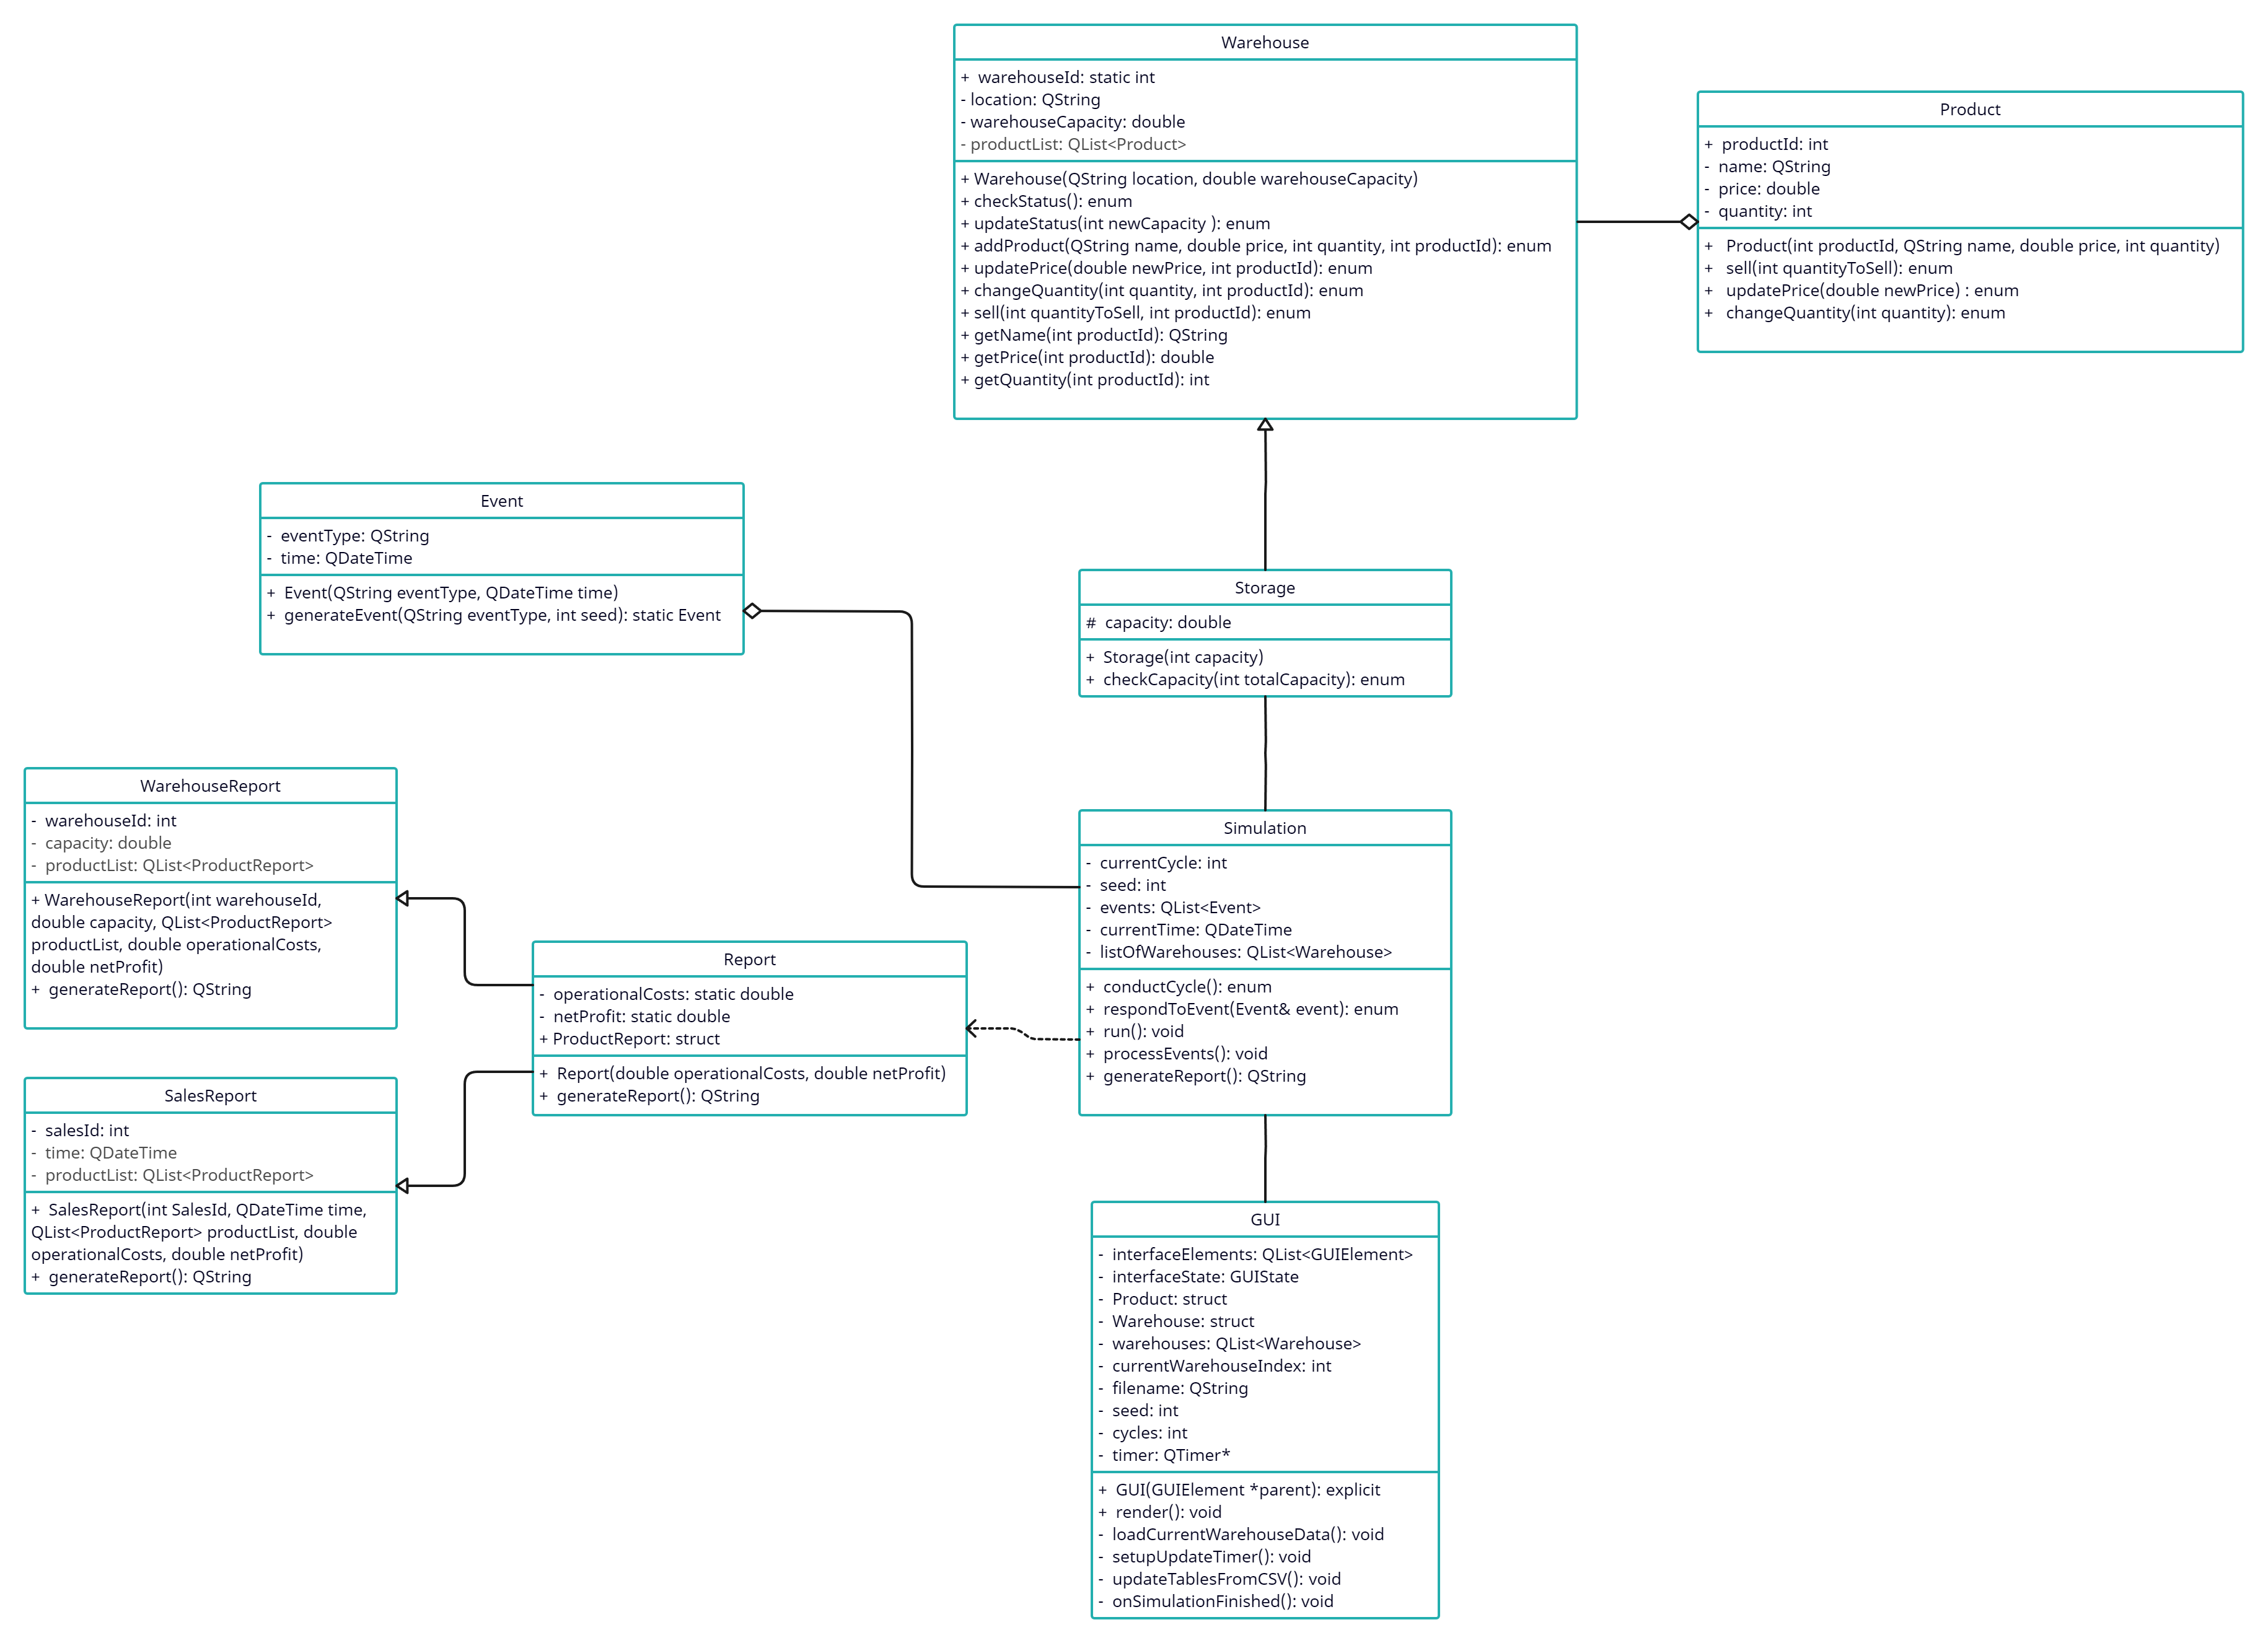
\includegraphics[scale=0.14]{Diagram klas.png}
    Figura 1: Diagram klas.
\end{center}

Opis diagramu klas dla symulacji domu towarowego w języku C++, który spełnia wymienione warunki:

\begin{enumerate}

    \item Klasa \textbf{Simulation} :
    \begin{itemize}
        \item \textbf{Atrybuty:} currentCycle, seed, currentTime, events, listOfWarehouses.
        \item \textbf{Metody:} conductCycle(), respondToEvent(Event\& event), run(), processEvents(), generateReport().
    \end{itemize}

    \item Klasa \textbf{Storage} :
    \begin{itemize}
        \item \textbf{Atrybuty:} capacity.
        \item \textbf{Metody:} checkCapacity(int totalCapacity).
    \end{itemize}

    \item Klasa \textbf{Warehouse} :
    \begin{itemize}
        \item \textbf{Atrybuty:} warehouseId, location, werehouseCapacity, productList.
        \item \textbf{Metody:} checkStatus(), updateStatus(int newCapacity), addProduct(QString name, double price, int quantity, int productId), updatePrice(double newPrice, int productId), changeQuantity(int quantity, int productId), sell(int quantityToSell, int productId), getName(int productId), getPrice(int productId), getQuantity(int productId).
    \end{itemize}

    \item Klasa \textbf{Product} :
    \begin{itemize}
        \item \textbf{Atrybuty:} productId, name, price, quantity.
        \item \textbf{Metody:} sell(int quantityToSell), updatePrice(double newPrice)
        changeQuantity(int quantity).
    \end{itemize}

    \item Klasa \textbf{Event} :
    \begin{itemize}
        \item \textbf{Atrybuty:} eventType, time.
        \item \textbf{Metody:} generateEvent().
    \end{itemize}

    \item Klasa \textbf{Report} :
    \begin{itemize}
        \item \textbf{Atrybuty:} operationalCosts, netProfit, ProductReport.
        \item \textbf{Metody:} generateReport().
    \end{itemize}

    \item Klasa \textbf{WarehouseReport} :
    \begin{itemize}
        \item \textbf{Atrybuty:} warehouseId, capacity, productList.
        \item \textbf{Metody:} generateReport().
    \end{itemize}

    \item Klasa \textbf{SalesReport} :
    \begin{itemize}
        \item \textbf{Atrybuty:} salesId, time, productList.
        \item \textbf{Metody:} generateReport().
    \end{itemize}

\item Klasa \textbf{GUI} :
    \begin{itemize}
        \item \textbf{Atrybuty:} interfaceElements, interfaceState, Product, Warehouse, warehouses, currentWarehouseIndex,
        filename, seed, cycles, timer.
        \item \textbf{Metody:} render(), loadCurrentWarehouseData(), setupUpdateTimer(), updateTablesFromCSV(),
        onSimulationFinished().
    \end{itemize}
    
\end{enumerate}


\textbf{Hermetyzacja} jest zastosowana poprzez ustawienie atrybutów jako prywatnych (\textit{private}) i dostęp do nich poprzez publiczne metody (\textit{public}).
\vspace{1pt}

\textbf{Dziedziczenie} jest reprezentowane przez klasę \textit{Warehouse}, która dziedziczy po klasie \textit{Storage}.
\vspace{1pt}

\textbf{Kompozycja} występuje, gdy \textit{Simulation} zawiera obiekty \textit{Warehouse}, które z kolei zawierają obiekty \textit{Product}.
\vspace{1pt}

\textbf{Agregacja} jest zastosowana w klasie \textit{Simulation} dla klasy \textit{Event}.
\vspace{1pt}

\textbf{Polimorfizm} może być reprezentowany przez różne typy zdarzeń, które są obsługiwane przez metodę \textit{generateReport()} w klasie \textit{Report}. Każde zdarzenie może mieć inną implementację tej metody, w zależności od jego typu.

\newpage

\subsection{Diagram obiektów}

\begin{center}
    \includegraphics[scale=0.14]{Diagram obiektów.png}
    Figura 2: Diagram obiektów.
\end{center}

Opis diagramu obiektów dla przykładowej symulacji domu towarowego w języku C++.

\begin{enumerate}

\item Obiekty klasy \textbf{Simulation}
\begin{itemize}
    \item \textbf{simulation}: \{ currentCycle: 5, events: [event1, event2], currentTime: "2023-04-05T14:00:00Z", seed: 100, listOfWarehouses: [warehouse1, warehouse2] \}
\end{itemize}

\item Obiekty klasy \textbf{Storage}
\begin{itemize}
    \item \textbf{storage1}: \{ capacity: 1000 \}
    \item \textbf{storage2}: \{ capacity: 500 \}
\end{itemize}

\item Obiekty klasy \textbf{Warehouse}
\begin{itemize}
    \item \textbf{warehouse1}: \{ warehouseId: 1, location: "Warszawa", capacity: 1000, productList: [product1, product2] \}
    \item \textbf{storage2}: \{ warehouseId: 2, location: "Kraków", capacity: 500, productList: [product3, product4] \}
\end{itemize}

\item Obiekty klasy \textbf{Product}
\begin{itemize}
    \item \textbf{product1}: \{ productId: 101, name: "Laptop", price: 3000, quantity: 50 \}
    \item \textbf{product2}: \{ productId: 102, name: "Phone", price: 2000, quantity: 100 \}
    \item \textbf{product3}: \{ productId: 103, name: "Tablet", price: 1500, quantity: 30 \}
    \item \textbf{product4}: \{ productId: 104, name: "Headphones", price: 300, quantity: 200 \}
\end{itemize}

\item Obiekty klasy \textbf{Event}
\begin{itemize}
    \item \textbf{event1}: \{ eventType: "Sale", time: "2023-04-05T10:00:00Z" \}
    \item \textbf{event2}: \{ eventType: "Delivery", time: "2023-04-06T10:00:00Z" \}
\end{itemize}

\item Obiekty klasy \textbf{Report}
\begin{itemize}
    \item \textbf{report1}: \{ operationalCosts: 5000, netProfit: 20000, Product: \{"Laptop", 3000, 50\} \}
\end{itemize}

\item Obiekty klasy \textbf{WarehouseReport}
\begin{itemize}
    \item \textbf{warehouseReport1}: \{ warehouseId: 1, capacity: 1000, productList: [productReport1, productReport2] \}
    \item \textbf{warehouseReport2}: \{ warehouseId: 2, capacity: 500, productList: [productReport3, productReport4] \}
\end{itemize}

\item Obiekty klasy \textbf{SalesReport}
\begin{itemize}
    \item \textbf{salesReport1}: \{ salesId: 201, time: "2023-04-Q1", productList: [productReport1, productReport2] \}
    \item \textbf{salesReport2}: \{ salesId: 202, time: "2023-04-Q2", productList: [productReport3, productReport4] \}
\end{itemize}

\item Obiekty klasy \textbf{GUI}
\begin{itemize}
    \item \textbf{gui}: \{ interfaceElements: [element1, element2], interfaceState: "ACTIVE", Product: \{"Laptop", 3000, 50\}, Warehouse: \{1, "Warszawa", 1000, products\}, warehouses: [warehouse1, warehouse2], currentWarehouseIndex = 1, filename: "settings.csv", seed: 100, cycles: 5 \}
\end{itemize}
    
\end{enumerate}

\subsection{Szczegółowy opis działania symulacji}

Użytkownik rozpoczyna symulację poprzez interfejs użytkownika \textbf{GUI} lub terminal, tworząc plik konfiguracyjny CSV oraz wywołując metodę \textit{run()} klasy \textbf{Simulation}. Ta metoda inicjuje główną pętlę symulacji, która będzie się wykonywać przez określoną liczbę cykli reprezentujących jednostki czasu zawartą w zmiennej \textit{currentCycle}. W każdym cyklu symulacji, metoda \textit{conductCycle()} jest wywoływana. Odpowiada ona za przetwarzanie zdarzeń zaplanowanych na bieżący cykl, które są przechowywane w atrybucie \textit{events}. \par
Zdarzenia takie jak przyjęcie nowego towaru, sprzedaż produktu lub zmiana zapotrzebowania są generowane losowo lub według harmonogramu. Są one tworzone przez metodę \textit{generateEvent()} klasy \textbf{Event} i dodawane do kolejki zdarzeń w \textbf{Simulation}.\par
Metoda \textit{respondToEvent()} klasy \textbf{Simulation} jest wywoływana, aby zareagować na każde zdarzenie. Może to obejmować aktualizację stanu magazynu, zamówienie nowego towaru czy przesunięcie zasobów.\par
Obiekty klasy \textbf{Warehouse}, które są częścią \textit{listOfWarehouses} w \textbf{Simulation}, są aktualizowane w odpowiedzi na zdarzenia. Metody takie jak \textit{checkStatus()} i \textit{updateStatus()} są używane do monitorowania i modyfikacji stanu magazynu.\par
Produkty reprezentowane przez obiekty klasy \textbf{Product} są sprzedawane i zarządzane poprzez metody takie jak \textit{sell(), updatePrice() i changeQuantity()}, które są wywoływane w odpowiedzi na zdarzenia sprzedaży.\par
Na koniec epoki, metoda \textit{generateReport()} klasy \textbf{Report} jest wywoływana, aby utworzyć raport z wynikami symulacji, takimi jak koszty operacyjne i zysk netto. Raporty mogą być szczegółowe dla magazynów \textbf{(WarehouseReport)} lub sprzedaży \textbf{(SalesReport)}.\par
Po zakończeniu określonej liczby cykli, symulacja kończy działanie, a użytkownik otrzymuje końcowy raport z wynikami.

\section{Implementacja}
\subsection{Użyte wzorce projektowe}

W projekcie Symulacji Domu Towarowego zastosowano szereg wzorców projektowych, które przyczyniają się do zwiększenia elastyczności, skalowalności oraz czytelności kodu źródłowego.

\begin{itemize}
    \item Wzorzec \textbf{Singleton} pozwolił na kontrolę nad tworzeniem instancji komponentów aplikacji.
    \item Wzorzec \textbf{Fabryka} ułatwił zarządzanie tworzeniem obiektów oraz pozwolił na elastyczne dostosowanie systemu do tworzenia różnorodnych instancji obiektów bez konieczności modyfikacji kodu.
    \item Wzorzec \textbf{Obserwator} był wykorzystywany do monitorowania zmian stanu obiektów i informowania o nich innych części symulacji, co pozwoliło zachować spójność stanu aplikacji i interfejsu użytkownika.
    \item Wzorzec \textbf{Strategia} umożliwił dynamiczną zmianę algorytmów działania obiektów, co jest kluczowe w symulatorze domu towarowego, gdzie różne scenariusze wymagają różnych decyzji (np. zakupienia produktu do magazynu).
\end{itemize}

\subsection{Zmiany w stosunku do pierwotnego projektu}

\begin{itemize}
    \item Konstruktory klas przyjmują parametry w celu ustawienia swoich atrybutów danymi już w momencie tworzenia obiektów. Poprawia to również czytelność kodu.
    \item W klasie \textbf{Warehouse} \textit{warehouseId} jest zmienną statyczną w celu lepszej kontroli nad unikalnością ID magazynu.
    \item Dodano dodatkowe metody umożliwiające operacje na obiektach klasy \textbf{Product} w celu utrzymania hierarchii klas oraz kompozycji powyższych klas.
    \item Atrybut \textit{capacity} klasy \textbf{Storage} został elementem typu Protected, aby umożliwić modyfikację ów atrybutu w dziedziczonych klasach.
    \item W klasie \textbf{Simulation} usunięto element \textit{eventAgenda}, ponieważ okazał się zbędnym atrybutem. Podobną informację można wyciągnąć bezpośrednio za pomocą metod klasy \textbf{Event}.
    \item W klasie \textbf{Simulation} zgodnie z propozycją prowadzącego zajęcia dodano atrybut \textit{seed}, który pozwala użytkownikowi określić ziarno generatora liczb losowych.
    \item W klasie \textbf{Report} zamiast działać bezpośrednio odwoływać się do klasy \textbf{Product}, zastosowano specjalnie przygotowaną strukturę \textit{ProductReport}. Poprawia to zgodność z wzorcem projektowym Obserwatora oraz nie narusza hierarchii klas.
    \item W klasie \textbf{GUI} dodano dodatkowe metody i atrybuty, aby implementacja nie polegała wyłącznie na slotach dostępnych w frameworku Qt oraz w celu przestrzegania zasad czystego kodu.
\end{itemize}

\subsection{Testowanie}
Do testowania użyto metod testowania jednostkowego za pomocą biblioteki Google Test oraz metodyki Test Driven Development. Scenariusze testowe obejmowały przetestowanie działania metod klas aplikacji np. poprawnej modyfikacji zadanego atrybutu czy poprawności zwracanej wartości. Obecny kod spełnia wszystkie przewidziane testy.

\begin{center}
    {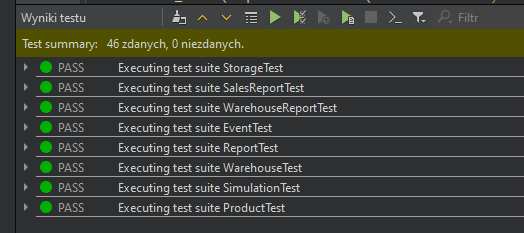
\includegraphics[]{wyniki_testow.png}}\\
    Figura 3: Wyniki testów jednostkowych symulacji.
\end{center}

\section{Przykładowy scenariusz}
\subsection{Uruchomienie z poziomu wiersza poleceń}
Aplikację można uruchomić z poziomu wiersza poleceń. W tym celu należy w katalogu z plikiem wykonywalnym uruchomić polecenie \textit{Warehouse-simulator.exe --nogui}. W trybie wiersza poleceń jest możliwe również wykorzystanie parametru \textit{--noconfig}, w celu ponownego uruchomienia poprzedniej symulacji bez konieczności przechodzenia etapu konfiguracji oraz \textit{--file} wraz z nazwą pliku z uprzednio przygotowaną konfiguracją poza katalogiem wykonywalnym.

\newpage

\begin{verbatim}
***************************
* 1. Add warehouse        *
* 2. Add product          *
* 3. Set number of cycles *
* 4. Set event seed       *
* 5. Undo last change     *
* 9. Exit configuration   *
***************************


Enter option: 1


Enter warehouse location: Wroclaw
Enter capacity of warehouse: 100
\end{verbatim}

\begin{center}
    Listing 1: Menu interfejsu wiersza poleceń.
\end{center}

\begin{verbatim}
Type,Location,Capacity,Name,Price,Quantity,Cycles,Seed
Warehouse,Wroclaw,100
Product,Laptop,1299.99,20
Product,Phone,599.99,80
Warehouse,Legnica,50
Product,Tablet,50,50
Cycles,,,,10
Seed,,,,,100
\end{verbatim}

\begin{center}
    Listing 2: Plik konfiguracyjny settings.csv
\end{center}

\newpage

\begin{verbatim}
Warehouse ID,Capacity
0,100
Product Name,Price,Quantity
Laptop,1299.99,14
Phone,599.99,74
Sales ID,Time
18,2024-06-09 19:25:23
Product Name,Price,Quantity Sold
Laptop,1299.99,14
Phone,599.99,74
Operational Costs,Net Profit
20779.8,681861
Warehouse ID,Capacity
1,50
Product Name,Price,Quantity
Tablet,50,38
Sales ID,Time
19,2024-06-09 19:25:23
Product Name,Price,Quantity Sold
Tablet,50,38
Operational Costs,Net Profit
20867.8,683673
\end{verbatim}

\begin{center}
    Listing 3: Fragment wyjścia programu. Plik SimulationReport.csv
\end{center}

\newpage

\subsection{Uruchomienie symulacji z poziomu interfejsu graficznego}
W tym celu należy uruchomić aplikację bez żadnych parametrów. W sekcji Settings można wybrać plik z konfiguracją lub wprowadzić ręcznie parametry symulacji oraz produkty w sekcji Warehouse. Następnie można uruchomic aplikację wybierając w menu Start simulation oraz zatwierdzając wybraną opcję przyciskiem Start simulation.

\begin{center}
    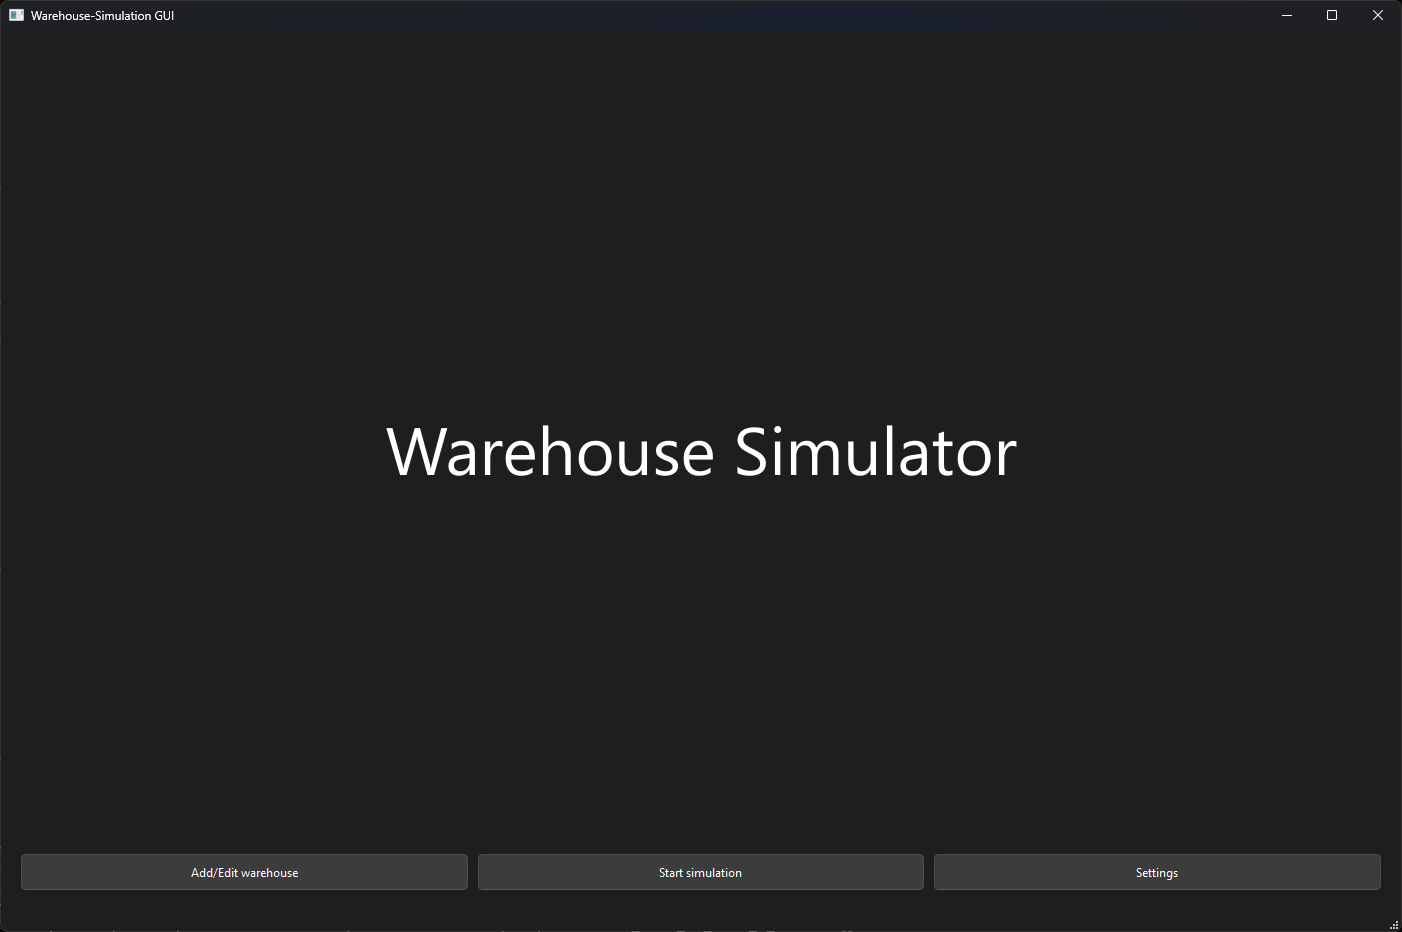
\includegraphics[scale=0.45]{menu.png}
    Figura 4: Ekran startowy aplikacji.
\end{center}
\begin{center}
    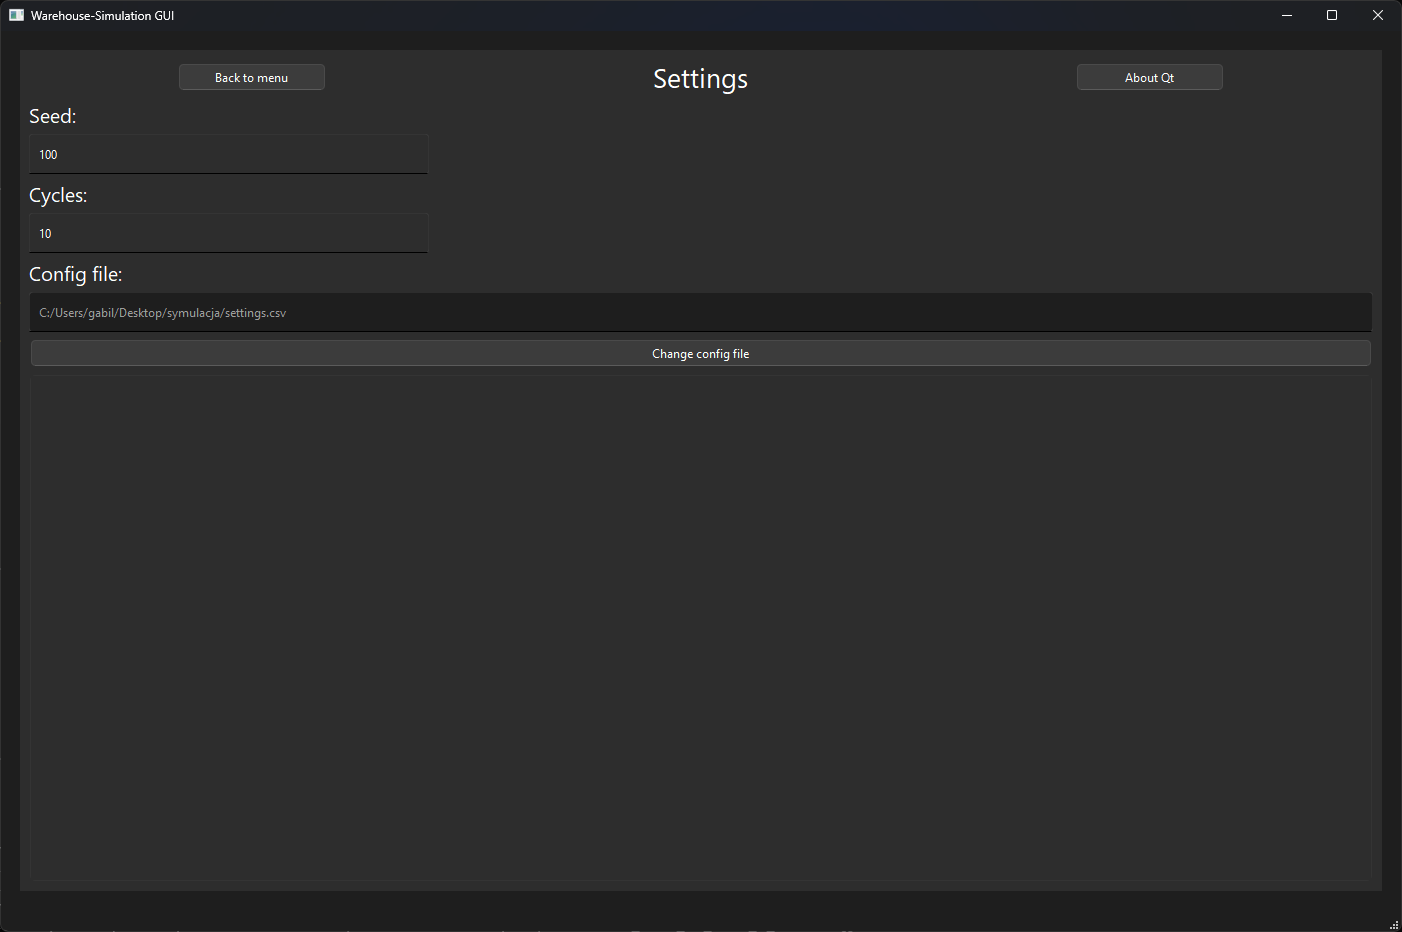
\includegraphics[scale=0.45]{ustawienia.png}
    Figura 5: Ekran ustawień parametrów symulacji.
\end{center}
\begin{center}
    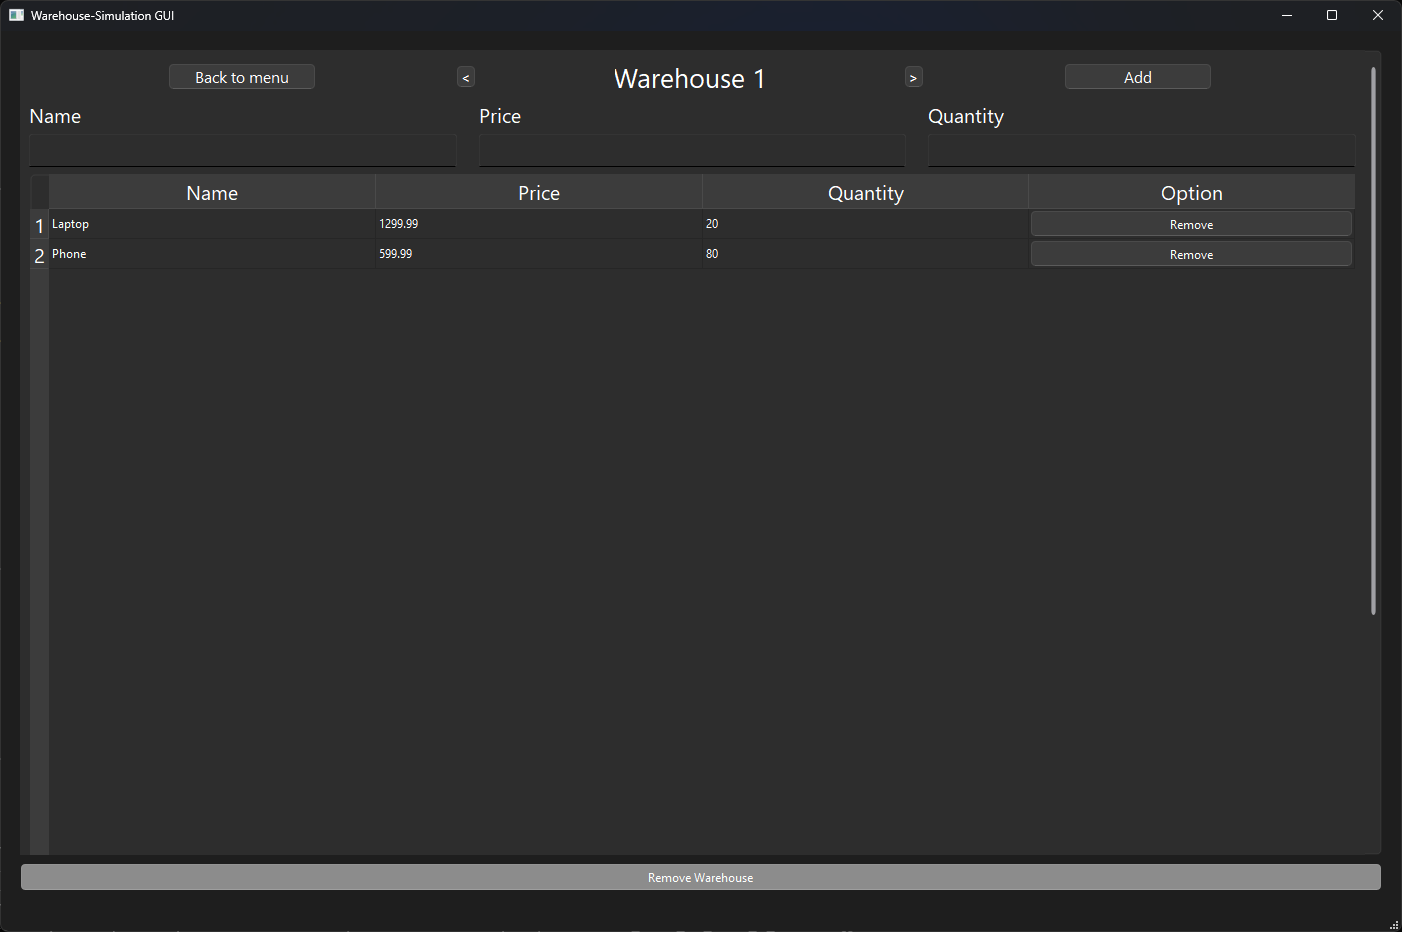
\includegraphics[scale=0.45]{warehouse1.png}
    Figura 6: Ekran ustawień pierwszego domu towarowego.
\end{center}
\begin{center}
    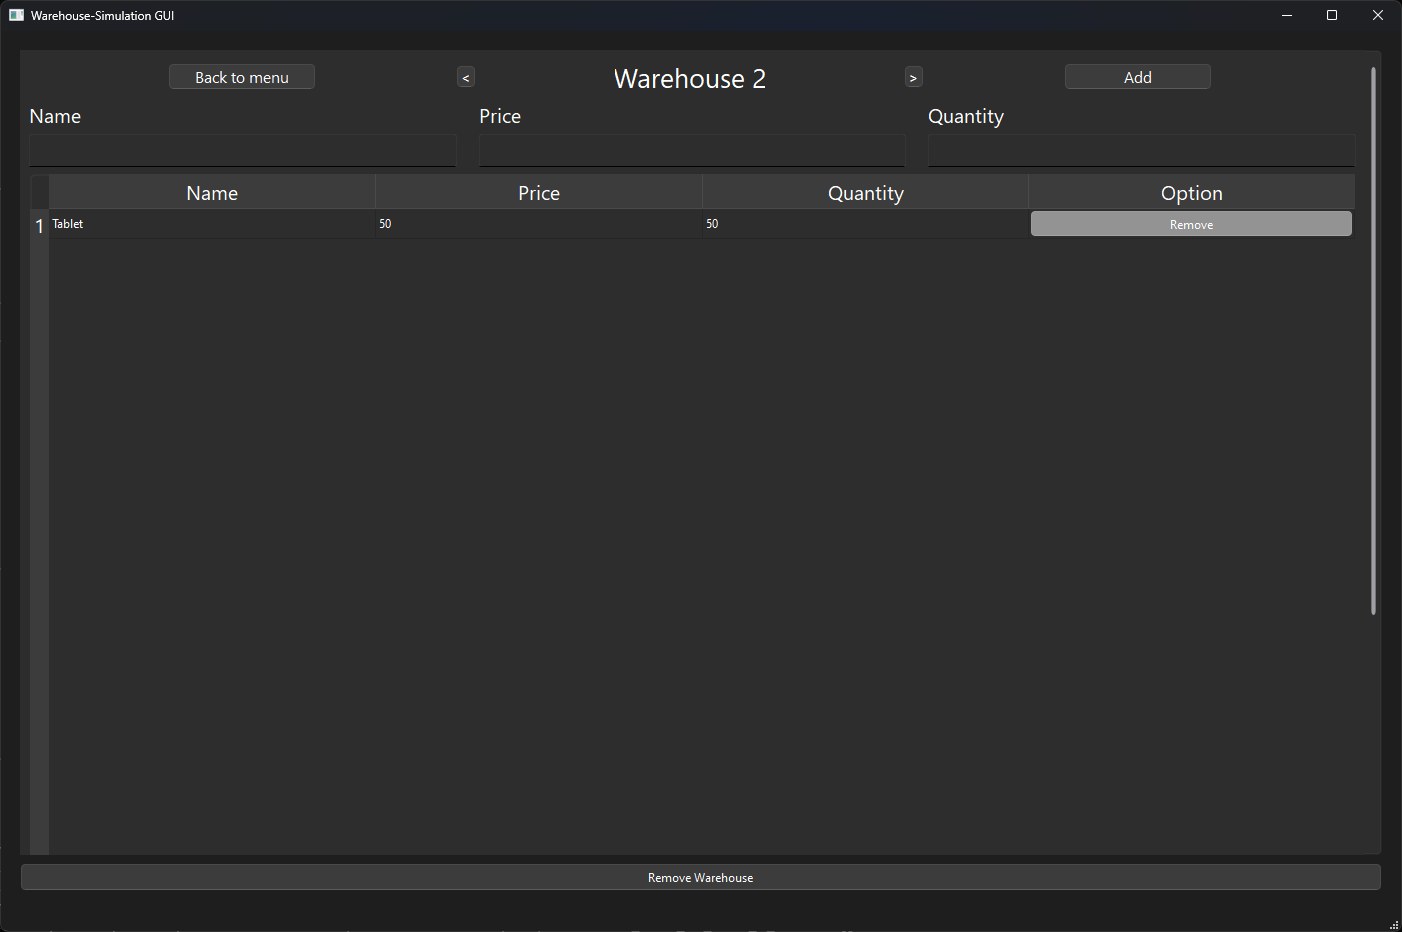
\includegraphics[scale=0.45]{warehouse2.png}
    Figura 7: Ekran ustawień drugiego domu towarowego.
\end{center}
\begin{center}
    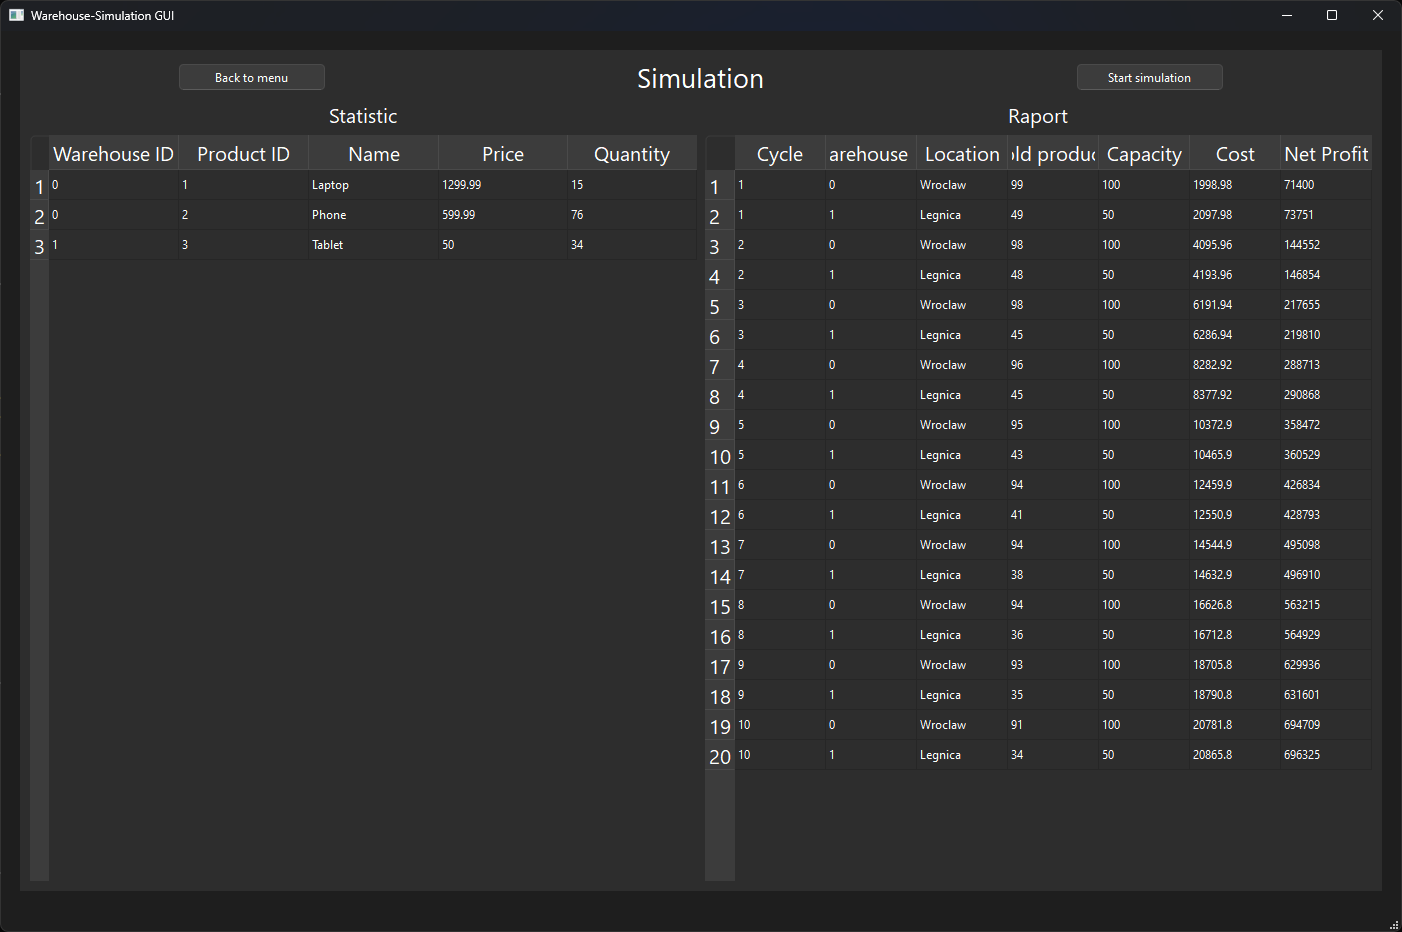
\includegraphics[scale=0.45]{wyniki.png}
    Figura 8: Ekran z wynikami symulacji.
\end{center}
\section{Podsumowanie}
\par W ramach projektu zrealizowano cele związane z poszerzaniem wiedzy i umiejętności w kilku kluczowych obszarach. Projekt umożliwił zapoznanie się z podstawami znormalizowanego języka modelowania UML, co jest fundamentalnym narzędziem w inżynierii oprogramowania. Ponadto, zdobyto wiedzę z zakresu inżynierii i metodologii programowania obiektowego, co jest niezbędne w projektowaniu nowoczesnych systemów.
\par Istotnym elementem było także poznanie podstawowych narzędzi programowania obiektowego na przykładzie języka C++, co pomogło w praktycznym zastosowaniu zdobytej wiedzy teoretycznej. W trakcie projektu rozwijano umiejętności stosowania technik obiektowych w programach, co pozwala na tworzenie bardziej modułowego i elastycznego kodu.
\par Konstrukcja kodu z wykorzystaniem hierarchii klas umożliwiła modelowanie złożonych problemów, a także praktyczne zastosowanie wzorców projektowych. Na koniec, umiejętność dokumentowania kodu źródłowego została ugruntowana poprzez szczegółowe opisanie implementacji, co jest kluczowe dla utrzymania i dalszego rozwoju oprogramowania.
\par W trakcie realizacji projektu napotkano na kilka wyzwań, takich jak synchronizacja pracy zespołu oraz integracja różnych modułów systemu. Problemy te rozwiązano poprzez regularne spotkania zespołu i zastosowanie narzędzi do zarządzania projektem, co zapewniło płynną realizację zadań.

\end{document}